\documentclass[12pt,a4paper]{article}
\usepackage[utf8]{inputenc}
\usepackage[russian]{babel}
\usepackage[OT1]{fontenc}
\usepackage{graphicx}
\usepackage{calc}
\usepackage[margin=15mm]{geometry}
\usepackage{cmap}

% условие без картинки
\newcommand{\task}[2]{
\hrule
\hbox to \textwidth {%
     \vrule
\parbox[t]{0.04\textwidth}{\smallskip \centering #1}%
     \vrule%
\hfill%
     \parbox[t]{0.93\textwidth}{\smallskip #2 \smallskip}\hfill%
\vrule
}
\hrule
    \pagebreak[2]
}

\newlength{\h}
\newsavebox{\taskbox}
\newlength{\x}
\newsavebox{\pictbox}

% условие с картинкой (картинка выравнивается по центру)
\newcommand{\taskpic}[3]{
\savebox{\taskbox}{\parbox[t]{0.93\textwidth-4.3cm}{\smallskip #2 \smallskip}}
\savebox{\pictbox}{\parbox[t]{4cm}{\smallskip \centering
     \vspace{0pt} #3 \smallskip}}
\h=\ht\taskbox
\advance\h\dp\taskbox
\x=\ht\pictbox
\advance\x\dp\pictbox
\hrule
\hbox to \textwidth {%
\vrule\parbox[t][\maxof{\h}{\x}][t]{0.04\textwidth}{ \smallskip
     \centering #1 }\vrule%
\hfill\parbox[t][\maxof{\h}{\x}][t]{0.93\textwidth-4.3cm}{\smallskip #2
     \smallskip}\hfill\vrule%
\hfill\parbox[t][\maxof{\h}{\x}][c]{4cm}{\hfil #3 \hfil}\hfill\vrule
}
\hrule
\pagebreak[2]
}
\pagestyle{empty}
\graphicspath{ {images/} }

\begin{document}
\begin{center}
\begin{Large}
\textsc{ГЦФО. 9 класс. 2014/15.}
\end{Large}
\end{center}
\taskpic{13}{Два одинаковых бруса скрепили за середины торцов одинаковыми нерастяжимыми нитями и положили на угол стола (см. рис.). Торцы выступают за края столешницы так, что нити не касаются стола. Коэффициент трения о вертикальную поверхность стола в 3~раза больше, чем о горизонтальную. Известно, что если поставить систему с начальным углом нити к горизонтали $\alpha < 45^\circ$ (см. рис.), то бруски начнут двигаться, тогда как если в начальный момент $\alpha \geqslant 45^\circ$, то система остается неподвижной. Найдите коэффициент трения о горизонтальную поверхность.}{
\begin{tikzpicture}[scale=0.25]
\draw[thick] (0,0)--(5,0)--(5,-5);
\draw[thick] (1.5,4)--(8,4)--(8,-3.5);
\draw[thick] (5,0)--(8,4);
\filldraw[fill=gray] (1,0) rectangle (3,2);
\filldraw[fill=gray] (3,0)--(6,4)--(6,6)--(3,2)--cycle;
\filldraw[fill=gray] (1,2)--(3,2)--(6,6)--(4,6)--cycle;
\filldraw[fill=gray] (5,-4) rectangle (7,-2);
\filldraw[fill=gray] (7,-4)--(10,0)--(10,2)--(7,-2)--cycle;
\filldraw[fill=gray] (5,-2)--(7,-2)--(10,2)--(8,2)--cycle;
\draw[thick] (2,1) node[circle,fill=black,inner sep=0,minimum size=0.1cm] {} --(6,-3) node[circle,fill=black,inner sep=0,minimum size=0.1cm] {};
\draw[thick,dashed] (5,5) node[circle,fill=black,inner sep=0,minimum size=0.1cm] {}--(9,1) node[circle,fill=black,inner sep=0,minimum size=0.1cm] {};
\draw[thick,dashed] (2,-3)--(6,-3);
\draw[thick] (4,-3) arc (180:135:2) node[midway,left] {$\alpha$};
\end{tikzpicture}
}
\taskpic{15}{На гладкой наклонной плоскости, составляющей с горизонтом угол $\alpha=30^\circ$, расположен массивный клин (см. рис.). На верхней горизонтальной поверхности клина лежит маленькая легкая шайба. Клин отпускают, и он начинает свободно соскальзывать вниз.
\begin{enumerate}
\item Определите величину и направление ускорения движения шайбы относительно наклонной плоскости.
\item Как выглядит движение шайбы в системе отсчета, связанной с клином?
\end{enumerate}
Масса шайбы много меньше массы клина. Трением пренебречь.}{
\begin{tikzpicture}
\draw[thick] (0,1.5)--(3,0);
\draw[thick,dashed] (0.5,0.5)--(2,0.5);
\filldraw[thick,fill=gray] (0.5,1.27)--(2.5,0.27)--(2.5,1.27)--cycle;
\filldraw[fill=black] (1.6,1.28) rectangle (1.8,1.38);
\draw[thick] (1.5,0.5) arc (180:153.5:0.5) node[midway,left] {$\alpha$};
\end{tikzpicture}
}
\taskpic{16}{Три одинаковых бревна, имеющих форму цилиндра, сложены так, как показано на рисунке. Какие минимальные коэффициенты трения бревен друг по другу и бревен по земле необходимы для того, чтобы система оставалась в покое?}{
\begin{tikzpicture}
\draw[thick,interface] (3,0)--(0,0);
\draw[thick] (1,0.5) circle [radius=0.5];
\draw[thick] (2,0.5) circle [radius=0.5];
\draw[thick] (1.5,1.366) circle [radius=0.5];
\end{tikzpicture}
}
\taskpic{18}{На примусе, расходующем $\mu = 0{,}1$~кг бензина в час, стоит котелок, в котором находится $m = 1$~кг воды. График зависимости тепловой мощности $P$, выделяемой в окружающую среду, от времени приведен на рисунке. Постройте график зависимости температуры воды в котелке от времени. Теплоемкость котелка $C = 800$~Дж/$^\circ$C, удельная теплоемкость воды $c_0 = 4200$~Дж/(кг$\cdot^\circ$C). Удельная теплота сгорания бензина $q = 43$~МДж/кг. Начальная температура воды $T=20^\circ$C. Принять, что в любой момент времени температура котелка и воды совпадают.}{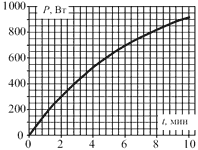
\includegraphics[width=4cm]{18}}
\task{19}{В морозильной камере, потребляющей из сети мощность 100~Вт, находится 20~кг воды при температуре 0$^\circ$C. За 1~час вся вода замерзла. Какое количество теплоты за это время выделилось в окружающую среду? Теплота плавления льда 330~кДж/кг. Считать, что в процессе замерзания температура льда остается постоянной, равной 0$^\circ$C.}
\taskpic{20}{Любознательный школьник разобрал нагревательный прибор. Оказалось, что схема прибора очень проста (см. рисунок). Школьник вынул все резисторы из схемы и обнаружил, что их сопротивления составляют $R_1=1$~Ом, $R_2=1$~Ом, $R_3=2$~Ом, $R_4=3$~Ом, $R_5=5$~Ом. Но он забыл, какой резистор на каком месте располагается в схеме. Помогите ему собрать прибор по старой схеме таким образом, чтобы его мощность была максимальной. Нагреватель работает от постоянного напряжения.}{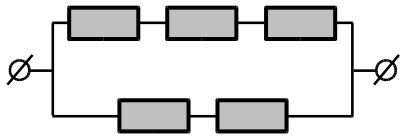
\includegraphics[width=4cm]{20}}
\end{document}
